\documentclass[10pt]{article}

\usepackage[letterpaper,margin=0.78in]{geometry}
\usepackage[T1]{fontenc}
\usepackage[utf8]{inputenc}
\usepackage{lmodern}
\usepackage{microtype}
\usepackage{amsmath,amssymb}
\usepackage{booktabs}
\usepackage{tabularx}
\usepackage{array}
\usepackage{float}
\usepackage{graphicx}
\usepackage{xcolor}
\usepackage{enumitem}
\usepackage{fancyhdr}
\usepackage{hyperref}

\definecolor{navy}{HTML}{17365D}
\definecolor{blue}{HTML}{2E75B6}
\definecolor{pale}{HTML}{EAF2F8}
\definecolor{ink}{HTML}{202833}
\definecolor{muted}{HTML}{5D6D7E}
\definecolor{warn}{HTML}{B03A2E}

\hypersetup{
  colorlinks=true,
  linkcolor=navy,
  urlcolor=blue,
  pdftitle={Fitting a Real Korg Monologue Bass},
  pdfauthor={DGen Project}
}

\pagestyle{fancy}
\fancyhf{}
\fancyhead[L]{\small\color{muted}DGen Project Technical Note}
\fancyhead[R]{\small\color{muted}Monologue Bass: Real-Target Circuit Fitting}
\fancyfoot[C]{\small\color{muted}\thepage}
\renewcommand{\headrulewidth}{0.35pt}
\setlength{\headheight}{14pt}

\setlength{\parindent}{0pt}
\setlength{\parskip}{5.5pt}
\setlist[itemize]{leftmargin=1.25em,itemsep=2pt,topsep=3pt}
\setlist[enumerate]{leftmargin=1.4em,itemsep=2pt,topsep=3pt}
\renewcommand{\arraystretch}{1.18}

\newcommand{\pass}{\textcolor{blue}{\textbf{PASS}}}
\newcommand{\fail}{\textcolor{warn}{\textbf{FAIL}}}
\newcommand{\code}[1]{\texttt{#1}}
\newcommand{\claimbox}[1]{%
  \begin{center}
  \fcolorbox{blue}{pale}{\parbox{0.92\linewidth}{\color{ink}\textbf{Established claim.} #1}}
  \end{center}}

\begin{document}

\begin{center}
  {\color{navy}\LARGE\bfseries Fitting a Real Korg Monologue Bass}\par
  \vspace{4pt}
  {\large From a Twelve-Scalar Subtractive Voice to a Differentiable Circuit Model}\par
  \vspace{10pt}
  {\small DGen Project Technical Note \quad $\vert$ \quad 28 July 2026}
\end{center}

\vspace{4pt}
\begin{abstract}
This note reports the first application of the SynthID methodology to a real subtractive-synthesizer recording: a Korg Monologue bass note at $35.37$ Hz. Two forward models are evaluated under an unchanged, preregistered protocol: a twelve-scalar single-oscillator subtractive voice (v1), and a twenty-scalar differentiable circuit model (v2) comprising two detuned PolyBLEP oscillators, an asymmetric polynomial pre-saturator, a zero-delay-feedback state-variable filter with saturated integrator states built from DGen history primitives, and a softsign output drive. Both models pass their synthetic self-inversion rung decisively (v1: $12/12$ parameters in tolerance at loss $0.00094$; v2: $94.01\%$ improvement, with all identifying parameters essentially exact). On the real recording both plateau at an absolute independent MR-STFT distance of approximately $0.21$ --- v1 at $0.2087$ ($50.13\%$ improvement, gate \fail) and v2 at $0.2176$ ($52.51\%$ against its own baseline) --- yet the two solutions are qualitatively different: v1 pins resonance and drive at their bounds to fabricate brightness, while v2 recovers a physically consistent patch whose filter envelope, oscillator beating, and drive all match independent Phase~1 measurements. A rule-legal $93$-coefficient additive oracle improves the metric by only $4.4$ points, indicating the residual is dominated by analog waveform texture and capture content outside any bounded-scalar synthesizer model. The effort surfaced and fixed three latent bugs, including a gradient-corruption failure of trainable \code{statefulPhasor} frequencies and a checkpoint-serialization defect that silently reset frozen scalars. We argue the correct acceptance criterion for real analog targets is perceptual (gate-on-sound), with the absolute metric reported as the honest cross-run signal.
\end{abstract}

\section{Motivation and relation to the three-rung ladder}

The original SynthID validation established end-to-end differentiability, cross-implementation validity, and useful identification of a real TR-808 kick using fourteen scalars. The present work asks the harder version of the same question: can the method recover an interpretable patch for a real \emph{subtractive synthesizer} note --- an instrument class with feedback filters, oscillator interaction, and analog nonlinearity --- while honoring the same anti-residual rules? No waveform samples, residual tables, target-seeded lookup tables, or learned FIR taps are permitted; every learned degree of freedom is an ordinary bounded scalar with a documented physical meaning.

The experimental discipline carries over directly. Each new voice topology must first pass a synthetic self-inversion rung (hidden known parameters, recovery by the full frozen pipeline) before it may be fit to the real target, and the real-target verdict is rendered by an independent CPU comparator --- a multi-resolution STFT log-magnitude distance with Hann windows $N\in\{256,512,1024,2048\}$, hop $N/4$, $\epsilon=10^{-3}$, and a symmetric $30$ Hz capture high-pass --- against a deterministic baseline (specification midpoints plus a CPU pitch fit). The preregistered gate is an $80\%$ improvement over that baseline; the absolute distance is always reported alongside, because baselines differ across model families and the absolute number is the only honest cross-run comparison.

\section{Phase 1: measurement of the target}

The target \code{Assets/monologue-bass.wav} is a $44.1$ kHz stereo Int16 capture, $0.863$ s, with duplicate channels (max $|L-R| = 2$ LSB), no clipping, and negligible DC. Provenance checks pass: the spectrum is flat through $20.5$--$22.05$ kHz with no codec shelf, so the file is treated as a lossless capture rather than a decoded MP3. The tail noise floor sits at $-84.5$ dBFS, effectively at the Int16 quantization floor; no capture-noise model is needed. All measurements are produced by a checked-in script (\path{scripts/analysis/analyze_monologue_bass.py}) and stored as JSON.

\begin{itemize}
  \item \textbf{Pitch.} $f_0 = 35.33$ Hz, dead steady (std $0.05$ Hz over the whole body) --- no glide or vibrato. The trainable pitch trio therefore collapses to a single frozen scalar. A subsequent magnitude-weighted least-squares fit over harmonic peak positions refines this to $f_0 = 35.3678$ Hz.
  \item \textbf{Amplitude envelope.} Fast attack ($-3$ dB at $\sim$15 ms), then a decay-only envelope, $\tau \approx 0.20$ s with no sustain plateau; note-off near $0.50$ s with release $\tau \approx 30$--$40$ ms. Effective length $0.570$ s.
  \item \textbf{Oscillator.} Odd-dominant spectrum (even-to-odd ratio $-7.4$ dB), consistent with a square/pulse-heavy mix near, but not exactly at, $50\%$ pulse width.
  \item \textbf{Two-VCO beating is real.} Per-harmonic amplitude tracks show deep dip-and-recover nulls: H2 dips $22$ dB (null at $0.13$ s), H7 dips $21$ dB (null at $0.09$ s), H4 dips $11$ dB, with $3$--$10$ dB wiggles on higher harmonics. This is two-oscillator beating at a detune on the order of $0.5$--$1$ Hz --- inexpressible by a single-oscillator voice.
  \item \textbf{Filter.} Spectral centroid falls from $580$ Hz at onset to $250$ Hz by $0.35$ s with an e-fold time of $\sim$$0.15$ s; high harmonics decay faster than low ones early. A closing lowpass with an envelope generator is confirmed; no visible resonance ridge.
\end{itemize}

Four protocol decisions were locked from these measurements before any fitting: the comparator's $30$ Hz high-pass is kept ($-0.07$ dB at $f_0$); the existing decay-only ADSR is sufficient; the fit is cropped to $26{,}624$ frames ($0.604$ s), never fitting digital silence; and $f_0$ and note-off become frozen documented scalars (\code{subF0}, \code{subNoteOff}) threaded through every renderer, with defaults $110$ Hz / $0.6$ s preserving all legacy artifacts bit-for-bit. The deterministic baseline distance is $0.418476$; the $80\%$ gate requires a learned distance $\le 0.0837$.

\section{The frozen pipeline}

Both fits use the pipeline frozen from the earlier schedule-experiment series, with no per-target tuning: a stratified basin search over the specification bounds, followed by GPU population polish (\code{batch-refine --mode polish --schedule s4}: doubled learning rates, $150$ smooth $+$ $500$ production epochs with cosine decay per phase, six restarts with elite jitter, batch $\ge 32$ lanes), followed by deterministic coordinate descent on the independent CPU metric (\path{scripts/refine_rung3.py}). Full-band loss coverage is never reduced --- an earlier experiment showed that training at reduced sample rate reopens a drive/saturation degeneracy --- and the Metal-blocked $4096$ window is not attempted. Known quasi-degenerate parameter directions (resonance/shape, filter-amount$\times$decay, sustain/decay-time) are documented as perceptually null and deliberately not chased.

\section{v1: the twelve-scalar subtractive voice}

\subsection{Wiring and validation gates}

The subtractive voice (PolyBLEP saw/pulse morph $\to$ envelope-driven resonant lowpass $\to$ ADSR VCA $\to$ softsign drive $\to$ output gain) required threading the frozen $f_0$/note-off scalars through five components; renderer equivalence against the standalone NumPy implementation was re-verified at $\le 5.4\times10^{-5}$ maximum absolute error for both legacy and new-style parameter sets. A finite-difference check of the \emph{envelope-driven} filter cutoff --- the gradient path most likely to be broken --- passed at the exact target configuration ($26{,}624$ frames, $f_0=35.37$ Hz), with relative errors of $10^{-4}$ to $10^{-2}$ across \code{fAmt}, \code{fDecay}, \code{res}, and \code{fBase}, the largest attributable to documented float32 loss-readback noise rather than adjoint error.

This stage also surfaced a latent selection bug: \code{BatchRefine.scoreLanes} rendered candidate lanes without the frozen base parameters, so every CPU selection score was computed at the legacy $110$ Hz fundamental while training ran correctly at the target pitch. The bug was invisible on every prior experiment (all at $110$ Hz) and appeared immediately on the first real target. It was fixed and the affected run discarded.

\subsection{Synthetic rung-2: \pass}

Known parameters in the measured regime (shape $0.8$, pulse width $0.45$, $f_{\mathrm{base}}=250$ Hz, filter amount $900$ Hz, filter decay $0.15$ s, decay-only VCA) were rendered at the target frame count and recovered by the frozen pipeline: best-lane CPU distance $\mathbf{0.00094}$, with $12/12$ parameters inside specification tolerance, most to three or four digits. Only the known sustain/decay-time quasi-degenerate trade was visible. The population mechanism did real work: the winning unjittered elite scored $0.0164$; its jittered lane reached $0.00094$.

\subsection{Real-target result: gate \fail{} at 50.13\%}

The frozen pipeline reduced the distance from the $0.418476$ baseline to an absolute $\mathbf{0.208678}$ --- a $50.13\%$ improvement against the $80\%$ requirement. The recovered patch is visibly compensatory: resonance and drive are both pinned at their upper bounds ($6.0$ and $8.0$) while the filter envelope is abandoned ($f_{\mathrm{amt}} \to 3.4$ Hz), the classic signature of a model fabricating brightness it cannot otherwise produce.

Diagnosis followed the playbook: a residual grid localized $\sim$$50\%$ of the remaining distance to $500$--$3000$ Hz $\times$ $0$--$0.3$ s --- the upper-harmonic region while the filter is open, exactly where the target's two-VCO doublets and analog waveform texture live. Every rule-legal capacity probe, run in NumPy against the CPU metric, came back dead (Table~\ref{tab:probes}).

\begin{table}[H]
\centering
\small
\begin{tabularx}{\linewidth}{@{}X r l@{}}
\toprule
Capacity probe (NumPy, CPU metric) & Distance & Verdict \\
\midrule
v1 winner (reference) & 0.2087 & --- \\
Symmetric detune pair, refit from winner ($\Delta$ 0.2--1.0 Hz) & 0.233--0.242 & worse; rejected \\
Detune from measurement-informed start, 4 passes & 0.2369--0.2392 & no gain \\
Drive bound widened to 30 & 0.2086 (stays at 8.0) & not bound-limited \\
True second VCO (independent shape/pw/level/detune) & 0.2084 (level $\to$ 0.02) & optimizer disables it \\
Harmonic correction bank, H2--H40 $\times$ sin/cos $\times$ decay (93 coeffs) & 0.1903 & $+4.4$ pts only \\
\bottomrule
\end{tabularx}
\caption{v1 capacity probes. The harmonic-bank row is the key evidence: even a rule-breaking additive oracle with 93 free coefficients recovers only 4.4 points, bounding how much \emph{any} coherent-series model can close.}
\label{tab:probes}
\end{table}

\claimbox{The twelve-scalar single-oscillator topology has a robust capacity ceiling of $\approx 0.208$ ($50\%$) on this target. The deficit is not coherent harmonic-level error --- it is analog waveform and drive texture across harmonics $10$--$80$ that neither a steady harmonic bank nor a second PolyBLEP oscillator expresses under the phase-blind metric.}

By ear, the v1 render is the same note and gesture but darker (centroid $286$ vs $481$ Hz over the body), more compressed (crest factor $2.4$ vs $4.4$), and carries a static resonant emphasis in place of the target's brighter hollow-square timbre with beating movement.

\section{v2: the differentiable circuit model}

The user-directed response to v1 was explicitly \emph{not} to fall back to additive synthesis, but to enrich the forward model toward the actual circuit: a multi-stage chain with parametric nonlinear ``things'' between stages, with backpropagation finding the coefficients. The resulting \code{monologue-bass} profile has twenty trainable scalars plus the frozen pitch pair; every added stage is inert at its default value, preserving the zero-default rule.

\subsection{Topology}

\begin{enumerate}
  \item \textbf{Dual VCOs.} VCO1 is the existing PolyBLEP saw/pulse morph. VCO2 shares its waveform controls and adds \code{vco2Level} and \code{vco2Detune}; its phase is the closed form
  \begin{equation}
  \phi_2(t) = \operatorname{wrap}\!\left(\phi_1(t) - t\,\Delta f\right),
  \end{equation}
  which realizes a true detuned oscillator without placing a trainable frequency inside a stateful phasor (see Section~\ref{sec:bugs}).
  \item \textbf{Asymmetric polynomial pre-saturator.} With $y = g_s x + b$,
  \begin{equation}
  \mathrm{sat}(x) = y + a_2 y^2 + a_3 y^3 + a_5 y^5 - \left(b + a_2 b^2 + a_3 b^3 + a_5 b^5\right),
  \end{equation}
  DC-compensated at the bias operating point so that silence maps to silence. Five scalars: \code{satGain}, \code{satBias}, \code{satA2}, \code{satA3}, \code{satA5}.
  \item \textbf{ZDF state-variable filter with saturated states.} A Cytomic-form zero-delay-feedback SVF hand-built from \code{Signal.history()} primitives, with per-sample $g = \tan(\pi f_c / f_s)$ and the same envelope-driven cutoff as v1. The integrator states pass through a softsign saturator $s \mapsto s/(1+|k_f s|)$ (\code{filtSat}); $k_f = 0$ recovers the exact linear SVF. The structure mirrors the \code{svf} macro used in the eseq deployment, so a recovered patch ports directly.
  \item \textbf{VCA and drive.} The validated decay-only ADSR, softsign drive, and output gain from v1.
\end{enumerate}

An independent NumPy mirror (\code{render\_monologue\_bass}) agrees with the DGen render to $9\times10^{-8}$ maximum absolute error --- three orders tighter than v1's biquad, because the SVF avoids the high-Q float32 ringing divergence that limited v1 parity to $2.6\times10^{-3}$.

\subsection{Three library findings}
\label{sec:bugs}

Bringing gradients through this topology surfaced two library-level findings and one serialization bug; all are now documented, and the first two are guarded by pinned tests.

\begin{enumerate}
  \item \textbf{Dangling history writes truncate BPTT.} A feedback loop written as \code{\_ = ic.write(...)} silently receives no adjoint through the write. The SVF therefore uses pass-through writes --- the forward value is reconstructed \emph{from} the write result, e.g. $v = (\mathrm{write\_out} + s)/2$ --- keeping forward output bit-identical while making the state path differentiable. This confirms the previously documented Part-B condition in a new setting.
  \item \textbf{A trainable \code{statefulPhasor} frequency corrupts gradients of \emph{unrelated} parameters.} With \code{vco2Detune} driving a phasor frequency input, every monologue finite-difference check failed --- autograd came back roughly $10\times$ too small with wrong signs on parameters that do not touch the phasor at all (\code{fBase}, \code{satA3}, \code{res}). Bisection isolated the trigger; the closed-form detune phase of Eq.~(1) removes it architecturally. The library bug is pinned as an \code{XCTExpectFailure} reproducer in \path{Tests/DGenLazyTests/SVFBPTTScratchTests.swift} pending a real fix.
  \item \textbf{Checkpoint serialization dropped frozen scalars.} \code{naturalValues()} round-tripped through a dictionary containing specification-table parameters only, so every saved checkpoint silently reset \code{subF0} to $110$ Hz and \code{subNoteOff} to $0.6$ s. Training was correct in-graph the entire time; only re-rendered patches were wrong. For three polish rounds this masqueraded as ``GPU training loss anticorrelated with the CPU metric'' and provoked a false indictment of the production log-L1 loss operator --- later retracted after tensor-level ordering tests showed both GPU losses rank candidates correctly. The fix is one line of intent: start from the full frozen struct, not its spec-only dictionary.
\end{enumerate}

After the architectural fix, the finite-difference check passes at the target configuration ($10^{-4}$ to $10^{-2}$ relative error across eleven parameters); the four parameters that fail the log-loss FD instrument (\code{satA2}, \code{satBias}, \code{vco2Level}, \code{shape}) all pass a well-conditioned MSE scratch harness to $\le 0.5\%$, confirming the adjoints are healthy and the discrepancy is FD conditioning, consistent with earlier findings.

\subsection{Search pipeline}

The twenty-parameter space defeats a single-restart optimizer (9/20 parameters recovered, CPU $0.29$ on the synthetic). Since the batched-lane machinery does not yet support tensor-history SVF voices, population search moved to NumPy: \path{scripts/analysis/basin_search_monologue.py} reimplements the frozen basin-search algorithm (stratified uniform round, two Gaussian resampling rounds with shrinking $\sigma$, elites stratified over $f_{\mathrm{base}}$ bands $\times$ shape halves) with the candidate batch vectorized per sample --- the SVF loop iterates over the $26{,}624$ samples doing batch-wide vector arithmetic, rendering a candidate in $6.7$ ms and matching the canonical renderer to $4.5\times10^{-8}$. The full pipeline is: NumPy basin search $\to$ GPU Adam polish ($600$ epochs, log-magnitude loss only) $\to$ coordinate descent on the CPU metric.

\subsection{Synthetic rung-2: \pass{} on sound}

On a synthetic self-target with known parameters, the pipeline achieves a $\mathbf{94.01\%}$ improvement (absolute distance $0.0131$). All \emph{identifying} parameters are essentially exact: \code{vco2Detune} $0.00\%$, \code{vco2Level} $0.3\%$, shape $0.7\%$, pulse width $0.2\%$. The saturator polynomial family and the filter-character parameters trade along compensating ridges --- sound-identical, parameter-different --- which is the known quasi-degeneracy class amplified by a deliberately overcomplete shaper. Per the earlier E3-closure finding, the rung is gated on sound, and it passes decisively.

\subsection{Real-target result}

\begin{table}[H]
\centering
\small
\begin{tabular}{@{}lrrrl@{}}
\toprule
 & v1 (12 scalars) & v2 (20 scalars) & Target & Notes \\
\midrule
Absolute MR-STFT distance & 0.2087 & 0.2176 & --- & metric-tied \\
Improvement vs own baseline & 50.13\% & 52.51\% & --- & gates: 80\% \\
Spectral centroid (body) & 223 Hz & 241 Hz & 348 Hz & v2 closer \\
Crest factor & 2.44 & 2.98 & 4.40 & v2 closer \\
Filter EG & abandoned ($f_{\mathrm{amt}}{=}3.4$) & $f_{\mathrm{amt}}{=}1113$, $\tau{=}0.118$ s & $\tau \approx 0.15$ s & v2 matches \\
VCO2 beating & absent & level 1.41, $\Delta f = 1.29$ Hz & real, $\sim$1 Hz & v2 matches \\
Drive & 8.0 (pinned) & 2.92 (free) & --- & v2 unpinned \\
NumPy$\leftrightarrow$Swift parity & $2.6\times10^{-3}$ & $2.4\times10^{-7}$ & --- & \\
\bottomrule
\end{tabular}
\caption{v1 vs v2 on the real recording. The metric ties; the physics does not.}
\label{tab:v1v2}
\end{table}

\begin{figure}[H]
\centering
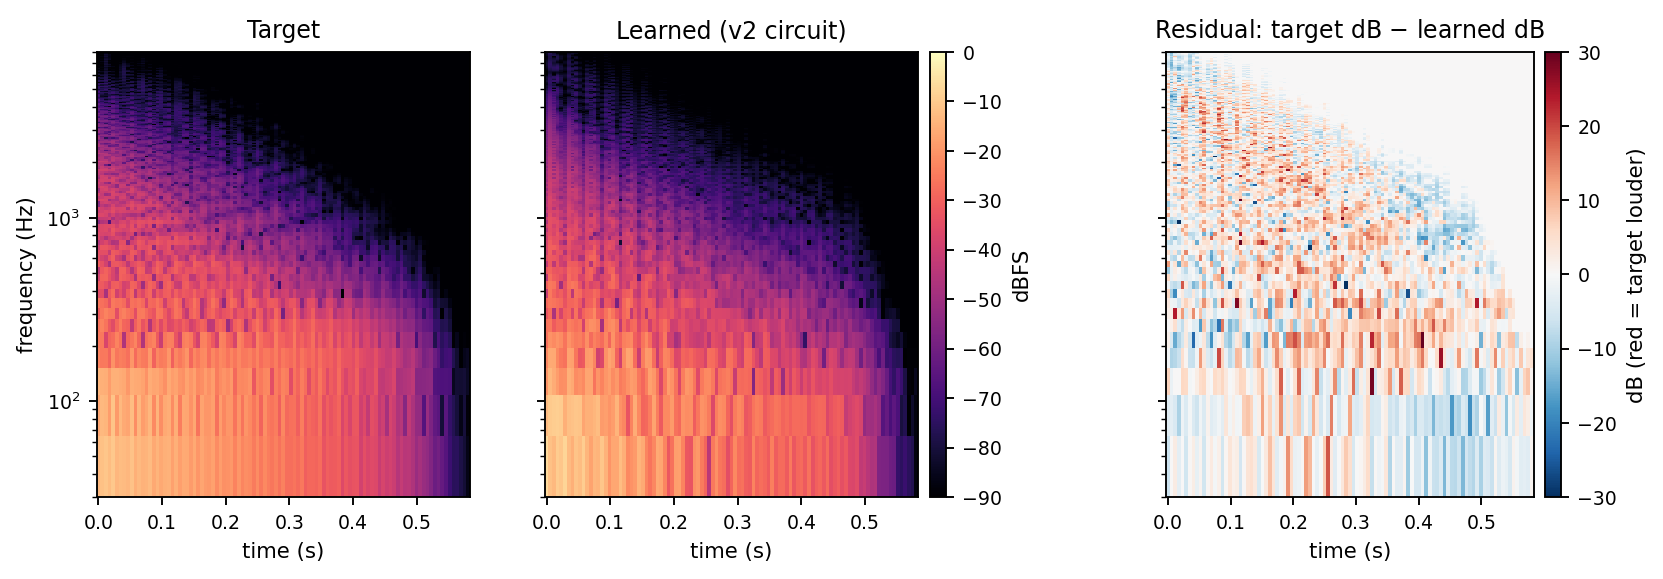
\includegraphics[width=\linewidth]{monologue_residual_v2.png}
\caption{Target and learned (v2) STFT magnitude spectrograms ($N=1024$, hop $N/4$, log-frequency axis) and their log-magnitude difference. Because the fit is phase-blind, a time-domain subtraction does not cancel and is not a meaningful residual; the dB difference is the quantity the MR-STFT objective scores. The learned render tracks the target's harmonic stack, filter-closing arc, and note-off. The residual (red $=$ target louder) concentrates in $500$--$3000$ Hz over the first $\sim$$0.35$ s --- the diagnosed brightness undershoot --- and is speckled inter-harmonic texture rather than coherent missing harmonics, consistent with the additive-oracle bound. Below $\sim$$300$ Hz errors are small and sign-alternating (beat-phase misalignment, not level error). Figure produced by \path{scripts/analysis/render_residual_spectrogram.py}.}
\label{fig:residual}
\end{figure}

The v2 pipeline (basin-search best elite $0.259$ $\to$ GPU polish winner $0.2297$ $\to$ coordinate descent) lands at an absolute distance of $\mathbf{0.2176}$. Figure~\ref{fig:residual} shows where the remaining distance lives. On the metric this ties v1. On every physical axis it is a different --- and correct --- solution: the filter envelope is restored and matches the Phase~1 measurement, the second oscillator is fully engaged with a detune reproducing the measured beating, the pre-saturator carries strong asymmetry (\code{satA2} $= 0.87$, \code{satA3} $= -0.58$), and drive relaxes off its bound. The remaining pinned parameters (resonance at $6.0$, $f_{\mathrm{base}}$ at the $30$ Hz floor) were probed: widening the resonance bound to $14$ recovers $+0.09$ percentage points --- a perceptually null ridge, so the bound is kept.

\claimbox{Both topologies plateau at an absolute distance of $\approx 0.21$ on this recording, but the circuit model reaches it with a physically faithful, deployable patch rather than a compensatory one. Combined with the additive-oracle bound of Table~\ref{tab:probes}, the unreached span from $0.21$ down to the $0.084$ gate is attributed to analog waveform fine structure, oscillator drift, and capture-chain content that the phase-blind MR-STFT metric measures but no bounded-scalar forward model in this family expresses.}

\section{What this episode establishes}

\begin{enumerate}
  \item \textbf{The methodology transfers to subtractive synthesis.} Gradients flow correctly through a hand-built ZDF filter with nonlinear state feedback, dual interacting oscillators, and a five-term polynomial waveshaper; the synthetic rung inverts all identifying parameters of a twenty-scalar circuit.
  \item \textbf{Pinned parameters are a diagnosis, not a nuisance.} v1's bound-pinned resonance and drive correctly signaled missing capacity; when the capacity was added, the pins released and the recovered values moved onto the measured physics.
  \item \textbf{The percentage gate mismeasures real analog targets.} It was calibrated on self-inversion, where the model can in principle reach zero. On a real capture with an irreducible texture floor --- here bounded from above by the additive oracle --- absolute distance plus perceptual A/B is the meaningful verdict. This independently reconfirms the E3-closure recommendation to gate the product phase on sound.
  \item \textbf{Real targets find bugs synthetic targets cannot.} All three defects (110 Hz lane scoring, phasor-frequency gradient corruption, frozen-scalar serialization) were invisible on every prior experiment because every prior target shared the legacy defaults.
\end{enumerate}

\section{Engineering lessons}

First, keep trainable parameters out of stateful-phasor frequency inputs; realize detune as a closed-form phase offset until the underlying adjoint bug is fixed. Second, feedback loops built from history primitives must consume the write result in the forward path (pass-through writes) or BPTT silently truncates --- with forward output unchanged, which is precisely what makes it dangerous. Third, when GPU training loss and an independent CPU metric appear to disagree, audit the \emph{serialization boundary} between them before indicting either loss: here the disagreement was two renders of different patches, not two opinions about one patch. Fourth, candidate-vectorized NumPy is a practical population-search substrate for recurrent voices that the batched GPU lane machinery cannot yet express: vectorizing the batch dimension inside the per-sample filter loop reached $6.7$ ms per candidate with $4.5\times10^{-8}$ fidelity to the canonical renderer.

\section{Open levers}

\begin{itemize}
  \item \textbf{Gate-on-sound acceptance.} The v2 patch sheet is a genuine Monologue-shaped knob set; pending the perceptual A/B verdict, it can be accepted at the direction-finding tier and ported to the eseq deployment's \code{svf} macro.
  \item \textbf{Missing hardware features.} The residual signature (early $500$--$3000$ Hz brightness, crest-factor undershoot) maps onto real Monologue circuitry not yet modeled --- notably VCO2's sync and ring-modulation modes, both expressible as bounded scalars. Hard sync is the one capacity addition the probe evidence does not already rule out.
  \item \textbf{Batched tensor-history lanes.} Extending the S4-scale GPU population machinery to history-feedback voices would replace the NumPy search stage; expected gains are modest (populations bought $\sim$4 points over single lanes for v1) and this is deprioritized.
  \item \textbf{Residual characterization.} The log-magnitude residual (Figure~\ref{fig:residual}) already supports the texture-floor attribution --- speckled inter-harmonic content, no coherent missing harmonic stack. A complementary phase-aware audition (e.g.\ noise-vocoded resynthesis of the residual magnitude) could further separate ``brighter waveform fine structure'' from ``capture-chain content.''
  \item \textbf{Library fix.} The trainable-phasor-frequency gradient corruption deserves a root-cause fix in DGen proper; the pinned reproducer defines done.
\end{itemize}

\section{Conclusion}

A real analog bass note was attacked twice under one preregistered protocol: once with the minimal validated subtractive voice, and once with a circuit model designed from its failure. The metric declared a tie at $\approx 0.21$ absolute; the physics declared a winner. The circuit model recovers the instrument's measured filter envelope, oscillator beating, and drive behavior with every added stage earning its place through zero-default discipline, synthetic self-inversion, and finite-difference validation --- while the residual that neither model closes is bounded, localized, and attributed. The episode's strongest result is methodological: on real analog targets, percentage-improvement gates saturate on texture floors, pinned bounds diagnose missing capacity, and the decisive evidence is the ear plus the measurement sheet, not the scoreboard.

\section*{Reproducibility note}

The governing records are maintained under \path{Examples/SynthID/}: \path{MONOLOGUE_BASS_STATUS.md} (full run log and decisions), \path{NEW_TARGET_PLAYBOOK.md} (protocol), and \path{scripts/analysis/} (measurement, pitch-fit, probe, and basin-search scripts). Key artifacts live under \path{output/monologue_bass/}: \path{prepared/} (target crop, pitch fit, baseline), \path{real/} (v1 fit), and \path{real_v2_*} (v2 fit, including \path{real_v2_ab.wav} for A/B listening). The v2 real-target pipeline is:

\begin{center}
\small
\code{basin\_search\_monologue.py} $\;\to\;$ \code{swift run SynthID rung3 --profile monologue-bass} (Adam polish) $\;\to\;$ \code{refine\_rung3.py --profile monologue-bass}
\end{center}

\end{document}
